% ============================================================
\chapter{Topologie Asym\'etrique en Informatique Th\'eorique}
\label{ch:informatique}
% ============================================================

En 1969, Dana Scott, confront\'e au probl\`eme de donner un sens math\'ematique au lambda-calcul de Church, cherche un espace $D$ isomorphe \`a son propre espace de fonctions continues $D \to D$. Les espaces classiques de la topologie de Hausdorff ne conviennent pas --- un tel isomorphisme y est impossible pour des raisons de cardinalit\'e. Scott d\'ecouvre que la solution r\'eside dans les \emph{treillis continus} munis de leur topologie de Scott, une topologie r\'esolument non-Hausdorff o\`u les ouverts repr\'esentent les propri\'et\'es \og observables \fg{} d'un calcul. Cette d\'ecouverte fonde la \emph{s\'emantique d\'enotationnelle}, le pont entre la logique des programmes et les math\'ematiques continues. Ce chapitre montre comment la topologie asym\'etrique --- les quasi-m\'etriques, les espaces $T_0$, la topologie de Scott --- constitue le langage naturel de l'informatique th\'eorique.

\begin{intuition}
La th\'eorie des domaines, n\'ee des travaux de Dana Scott dans les ann\'ees 1960--70,
fournit un mod\`ele math\'ematique pour la s\'emantique d\'enotationnelle des langages de
programmation. L'id\'ee centrale est que les \'el\'ements d'un domaine repr\'esentent des
\og{}niveaux d'information\fg partiels, et l'ordre refl\`ete le raffinement de
l'information. La topologie de Scott, qui est non-Hausdorff, capture exactement les
propri\'et\'es d'observabilit\'e dans un programme. Ce chapitre pr\'esente ces applications
de la topologie non-Hausdorff en informatique th\'eorique.
\end{intuition}

% ------------------------------------------------------------
\section{Domaines de Scott et s\'emantique d\'enotationnelle}
% ------------------------------------------------------------

\begin{definition}[Ensemble dirig\'e et dcpo]
\index{dcpo}
\index{ensemble dirig\'e}
Un sous-ensemble $D$ d'un ensemble ordonn\'e $(P, \leq)$ est \emph{dirig\'e} s'il est non
vide et si pour tous $x, y \in D$, il existe $z \in D$ tel que $x \leq z$ et $y \leq z$.
Un \emph{dcpo} (directed-complete partial order) est un ensemble ordonn\'e dans lequel
toute partie dirig\'ee admet un supremum.
\end{definition}

\begin{definition}[Topologie de Scott]
\index{topologie de Scott}
Soit $(P, \leq)$ un dcpo. Un sous-ensemble $U \subseteq P$ est \emph{Scott-ouvert} si~:
\begin{enumerate}
  \item $U$ est une partie haute~: $x \in U$ et $x \leq y$ impliquent $y \in U$~;
  \item $U$ est inaccessible par suprema dirig\'es~: si $D$ est dirig\'e et
    $\bigvee D \in U$, alors $D \cap U \neq \emptyset$.
\end{enumerate}
\end{definition}

\begin{proposition}
Les ouverts de Scott sur un dcpo $P$ forment une topologie. Cette topologie est $T_0$
et son ordre de sp\'ecialisation co\"incide avec l'ordre $\leq$ de $P$.
\end{proposition}

\begin{proof}
L'ensemble $P$ et $\emptyset$ sont Scott-ouverts. L'intersection finie de Scott-ouverts
est Scott-ouverte~: la condition de partie haute est pr\'eserv\'ee par intersection, et si
$\bigvee D \in U_1 \cap U_2$, alors $D \cap U_1$ est cofinal dans $D$, et
$D \cap U_1 \cap U_2$ est non vide. La r\'eunion quelconque de Scott-ouverts est
clairement Scott-ouverte.

Pour l'ordre de sp\'ecialisation~: $x \leq y$ dans l'ordre de $P$ si et seulement si
tout ouvert contenant $x$ contient $y$, ce qui est exactement la d\'efinition de l'ordre
de sp\'ecialisation.
\end{proof}

% Diagramme de Hasse du domaine plat des bool\'eens
\begin{center}
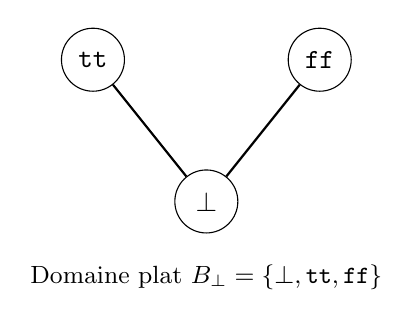
\begin{tikzpicture}[scale=1.2, every node/.style={circle, draw, minimum size=8mm, inner sep=1pt}]
  % Noeuds
  \node (bot) at (0,0) {$\bot$};
  \node (tt) at (-1.2,1.5) {$\mathtt{tt}$};
  \node (ff) at (1.2,1.5) {$\mathtt{ff}$};
  % Arêtes du diagramme de Hasse
  \draw[thick] (bot) -- (tt);
  \draw[thick] (bot) -- (ff);
  % L\'egende
  \node[draw=none, rectangle, minimum size=0pt] at (0,-0.8)
    {\small Domaine plat $\mathbb{B}_\bot = \{\bot, \mathtt{tt}, \mathtt{ff}\}$};
\end{tikzpicture}
\end{center}

\begin{definition}[Fonction Scott-continue]
\index{fonction Scott-continue}
Soient $(P, \leq_P)$ et $(Q, \leq_Q)$ deux dcpos. Une fonction $f\colon P \to Q$ est
\emph{Scott-continue} si elle est croissante et pr\'eserve les suprema dirig\'es~: pour
toute partie dirig\'ee $D \subseteq P$,
\[
  f\!\left(\bigvee D\right) = \bigvee f(D).
\]
\end{definition}

\begin{proposition}
Une fonction entre dcpos est Scott-continue si et seulement si elle est continue pour les
topologies de Scott.
\end{proposition}

\begin{theoreme}[Cat\'egorie des dcpos]
La cat\'egorie $\mathbf{DCPO}$ dont les objets sont les dcpos et les morphismes les
fonctions Scott-continues est cart\'esienne ferm\'ee. L'espace des fonctions
$[P \to Q]$ est le dcpo des fonctions Scott-continues de $P$ dans $Q$, ordonn\'e
point par point.
\end{theoreme}

\begin{proof}[Esquisse de preuve]
Le point cl\'e est de montrer que $[P \to Q]$, muni de l'ordre point par point
($f \leq g \iff \forall x,\, f(x) \leq g(x)$), est un dcpo. Si $(f_i)_{i \in I}$
est une famille dirig\'ee dans $[P \to Q]$, on d\'efinit $f = \bigvee f_i$ par
$f(x) = \bigvee_i f_i(x)$~; la Scott-continuit\'e de $f$ se v\'erifie en utilisant
la commutation des suprema dirig\'es. Pour la fermeture cart\'esienne, on doit
montrer que l'\'evaluation $\mathrm{ev} \colon [P \to Q] \times P \to Q$ est
Scott-continue~: si $U$ est Scott-ouvert dans $Q$, alors $\mathrm{ev}^{-1}(U)$ est
Scott-ouvert dans $[P \to Q] \times P$. Ceci d\'ecoule du fait que l'image
r\'eciproque d'un Scott-ouvert par l'\'evaluation est une r\'eunion de rectangles de
la forme $\{f : f(x) \in U\} \times V$, chacun \'etant Scott-ouvert.
Voir~\textsc{Abramsky--Jung},
\emph{Domain Theory}, Handbook of Logic in Computer Science, vol.~3, 1994.
\end{proof}

% ------------------------------------------------------------
\section{Domaines pour le lambda-calcul}
% ------------------------------------------------------------

\begin{definition}[Domaine continu]
\index{domaine continu}
Un dcpo $D$ est un \emph{domaine continu} si pour tout $x \in D$,
\[
  {\Downarrow} x = \{ a \in D : a \ll x \}
\]
est dirig\'e et $x = \bigvee {\Downarrow} x$, o\`u $a \ll x$ signifie que $a$ est
\emph{bien en dessous} de $x$ (compact relativement \`a $x$).
\end{definition}

\begin{theoreme}[Mod\`ele de Scott du lambda-calcul non typ\'e]
\label{thm:scott-model}
Il existe un domaine continu $D_\infty$ tel que
\[
  D_\infty \cong [D_\infty \to D_\infty]
\]
dans la cat\'egorie des domaines continus avec fonctions Scott-continues. Un tel domaine
fournit un mod\`ele de la s\'emantique d\'enotationnelle du lambda-calcul non typ\'e.
\end{theoreme}

\begin{proof}[Id\'ee de la preuve]
On construit $D_\infty$ comme limite projective d'une suite
$D_0 \leftarrow D_1 \leftarrow D_2 \leftarrow \cdots$ o\`u $D_0 = \{\bot\}$ et
$D_{n+1} = [D_n \to D_n]$, les fl\`eches \'etant des r\'etractions (paires
projection/section). La limite projective dans $\mathbf{DCPO}$ est un dcpo dont les
\'el\'ements sont les suites coh\'erentes $(x_0, x_1, \ldots)$ o\`u
$\pi_n(x_{n+1}) = x_n$. L'isomorphisme $D_\infty \cong [D_\infty \to D_\infty]$
d\'ecoule de la continuit\'e du foncteur $[\cdot \to \cdot]$ sur les limites projectives.
\end{proof}

\begin{intuition}
Le mod\`ele de Scott r\'esout un probl\`eme fondamental~: en th\'eorie na\"ive des ensembles,
il n'existe pas d'ensemble $D$ tel que $D \cong D^D$ (par un argument de cardinalit\'e,
sauf si $D$ est un singleton). En passant aux dcpos et aux fonctions continues, on
\'echappe \`a cette contrainte car $[D \to D]$ ne contient que les fonctions continues,
pas toutes les fonctions.
\end{intuition}

\begin{definition}[Interpr\'etation d\'enotationnelle]
\index{s\'emantique d\'enotationnelle}
Dans un mod\`ele de Scott $D_\infty$, chaque terme clos $M$ du lambda-calcul re\c{c}oit
une interpr\'etation $\llbracket M \rrbracket \in D_\infty$~:
\begin{itemize}
  \item $\llbracket x \rrbracket_\rho = \rho(x)$ o\`u $\rho$ est un environnement~;
  \item $\llbracket \lambda x.\, M \rrbracket_\rho = d \mapsto \llbracket M \rrbracket_{\rho[x \mapsto d]}$~;
  \item $\llbracket M N \rrbracket_\rho = \llbracket M \rrbracket_\rho (\llbracket N \rrbracket_\rho)$.
\end{itemize}
\end{definition}

% ------------------------------------------------------------
\section{Treillis continus et th\'eorie des langages}
% ------------------------------------------------------------

\begin{definition}[Treillis continu]
\index{treillis continu}
Un treillis complet $L$ est \emph{continu} s'il est un domaine continu, c'est-\`a-dire
si pour tout $x \in L$, $x = \bigvee \{a \in L : a \ll x\}$.
\end{definition}

\begin{theoreme}[Th\'eor\`eme de caract\'erisation de Lawson]
Un treillis complet $L$ est continu si et seulement si la fonction
$x \mapsto {\Downarrow} x$ est un isomorphisme de $L$ sur un sous-treillis du treillis
des id\'eaux de la base de $L$.
\end{theoreme}

\begin{proposition}[Treillis continus et types]
Dans la s\'emantique d\'enotationnelle~:
\begin{itemize}
  \item Les types de base (entiers, bool\'eens) sont interpr\'et\'es par des domaines
    alg\'ebriques plats (domaines avec \'el\'ement $\bot$ et \'el\'ements maximaux incomparables).
  \item Le type fonction $A \to B$ est interpr\'et\'e par $[D_A \to D_B]$.
  \item Les types r\'ecursifs $T = F(T)$ sont interpr\'et\'es par des solutions d'\'equations
    de domaines, obtenues comme limites projectives.
\end{itemize}
\end{proposition}

% ------------------------------------------------------------
\section{Powerdomaines}
% ------------------------------------------------------------

\begin{definition}[Powerdomaines]
\index{powerdomain}
Soit $D$ un domaine. Les \emph{powerdomaines} \'etendent $D$ pour mod\'eliser le
non-d\'eterminisme. Il en existe trois variantes, correspondant \`a trois observations
diff\'erentes~:
\end{definition}

\begin{definition}[Powerdomain de Hoare (inf\'erieur)]
\index{powerdomain!Hoare}
Le \emph{powerdomain de Hoare} $\mathcal{H}(D)$ est le dcpo des ferm\'es non vides de $D$
(dans la topologie de Scott), ordonn\'e par~:
\[
  A \leq_H B \quad \Longleftrightarrow \quad A \subseteq {\downarrow} B.
\]
Intuitivement, $A \leq_H B$ signifie que tout r\'esultat possible de $A$ est approxim\'e
par un r\'esultat de $B$. Cela capture la \og{}correction partielle\fg (s\^uret\'e).
\end{definition}

\begin{definition}[Powerdomain de Smyth (sup\'erieur)]
\index{powerdomain!Smyth}
Le \emph{powerdomain de Smyth} $\mathcal{S}(D)$ est l'ensemble des compacts satur\'es
non vides de $D$, ordonn\'e par inclusion inverse~:
\[
  Q_1 \leq_S Q_2 \quad \Longleftrightarrow \quad Q_2 \subseteq Q_1.
\]
Cela capture la \og{}terminaison\fg (vivacit\'e)~: $Q_1 \leq_S Q_2$ signifie que
l'ensemble des comportements possibles se r\'etr\'ecit.
\end{definition}

\begin{definition}[Powerdomain de Plotkin (convexe)]
\index{powerdomain!Plotkin}
Le \emph{powerdomain de Plotkin} $\mathcal{P}\ell(D)$ combine les deux ordres~:
\[
  A \leq_P B \quad \Longleftrightarrow \quad A \leq_H B \text{ et } A \leq_S B.
\]
C'est l'ordre d'Egli-Milner. Il capture \`a la fois la correction partielle et la
terminaison.
\end{definition}

\begin{theoreme}[Propri\'et\'es des powerdomaines]
Soit $D$ un domaine continu.
\begin{enumerate}
  \item $\mathcal{H}(D)$ est un dcpo (sous des hypoth\`eses l\'eg\`eres).
  \item $\mathcal{S}(D)$ est un dcpo si $D$ est coh\'erent (intersection de compacts
    satur\'es est compact satur\'e).
  \item Si $D$ est un domaine de Scott (domaine continu \`a base d\'enombrable), les trois
    powerdomaines sont des domaines continus.
\end{enumerate}
\end{theoreme}

\begin{exemple}
Consid\'erons le domaine plat des bool\'eens $\mathbb{B}_\bot = \{\bot, \mathtt{true},
\mathtt{false}\}$. Alors~:
\begin{itemize}
  \item $\mathcal{H}(\mathbb{B}_\bot)$ contient les ferm\'es~: $\{\bot\}$,
    $\{\bot, \mathtt{true}\}$, $\{\bot, \mathtt{false}\}$,
    $\{\bot, \mathtt{true}, \mathtt{false}\}$.
  \item $\mathcal{S}(\mathbb{B}_\bot)$ contient les compacts satur\'es~:
    $\mathbb{B}_\bot$, $\{\mathtt{true}\}$, $\{\mathtt{false}\}$,
    $\{\mathtt{true}, \mathtt{false}\}$.
\end{itemize}
\end{exemple}

% ------------------------------------------------------------
\section{Mod\`eles topologiques du calcul}
% ------------------------------------------------------------

\begin{definition}[Espace effectivement pr\'esent\'e]
\index{espace effectivement pr\'esent\'e}
Un domaine $D$ est \emph{effectivement pr\'esent\'e} s'il poss\`ede une base d\'enombrable
$(b_n)_{n \in \N}$ telle que les relations $b_n \leq b_m$ et $b_n \ll b_m$ soient
d\'ecidables (semi-d\'ecidables pour $\ll$).
\end{definition}

\begin{theoreme}[\'Equivalence calculabilit\'e--continuit\'e]
Sur un domaine effectivement pr\'esent\'e $D$, les fonctions calculables $D \to D$
(au sens de la th\'eorie de la calculabilit\'e de Type~2) co\"incident avec les fonctions
Scott-continues effectivement donn\'ees.
\end{theoreme}

\begin{proposition}[Espaces de noms et domaines]
Le domaine de B\"ohm $\mathcal{B}$ des arbres de B\"ohm du lambda-calcul est un domaine
continu tel que~:
\begin{itemize}
  \item Les \'el\'ements finis sont les arbres de B\"ohm finis (avec $\bot$ aux feuilles).
  \item L'ordre est le raffinement de l'information~: $t \leq s$ si $s$ est obtenu en
    rempla\c{c}ant certains $\bot$ de $t$ par des sous-arbres.
  \item La topologie de Scott capture exactement l'observation par contextes de t\^ete.
\end{itemize}
\end{proposition}

\begin{theoreme}[Ad\'equation et compl\'etude]
Pour le lambda-calcul pur, la s\'emantique d\'enotationnelle dans un domaine de Scott
continu est~:
\begin{enumerate}
  \item \emph{Ad\'equate}~: si $\llbracket M \rrbracket \leq \llbracket N \rrbracket$,
    alors $M$ est approch\'e par $N$ au sens op\'erationnel.
  \item \emph{Compl\`ete} pour les mod\`eles filtrables~: l'ordre d\'enotationnel
    co\"incide avec le pr\'eordre op\'erationnel.
\end{enumerate}
\end{theoreme}

\begin{formules}[title=\textbf{Correspondance topologie--informatique}]
\begin{center}
\renewcommand{\arraystretch}{1.3}
\begin{tabular}{|l|l|}
\hline
\textbf{Concept topologique} & \textbf{Concept informatique} \\
\hline
Ouvert de Scott & Propri\'et\'e semi-d\'ecidable \\
Ferm\'e de Scott & Propri\'et\'e v\'erifiable \`a la limite \\
Compact satur\'e & Propri\'et\'e co-semi-d\'ecidable \\
Fonction continue & Programme (fonction calculable) \\
Topologie $T_0$ & Distinguabilit\'e observationnelle \\
Point $\bot$ & Divergence / non-terminaison \\
Supremum dirig\'e & Limite d'approximations finies \\
\hline
\end{tabular}
\end{center}
\end{formules}

% ------------------------------------------------------------
\section{Exercices}
% ------------------------------------------------------------

\begin{exercice}
Montrer que la topologie de Scott sur $(\N, \leq)$ est la topologie cofinie sur $\N$.
\end{exercice}

\begin{exercice}
Soit $D = \N \cup \{\infty\}$ muni de l'ordre usuel. D\'eterminer la topologie de Scott,
v\'erifier qu'elle est sobre et localement compacte, et calculer les compacts satur\'es.
\end{exercice}

\begin{exercice}
Montrer que l'espace $[D \to D]$ des fonctions Scott-continues d'un dcpo $D$ dans
lui-m\^eme, muni de l'ordre point par point, est un dcpo. En d\'eduire que la cat\'egorie
$\mathbf{DCPO}$ est cart\'esienne ferm\'ee.
\end{exercice}

\begin{exercice}
Soit $D$ le domaine plat des entiers $\N_\bot$. D\'ecrire explicitement les \'el\'ements
du powerdomain de Hoare $\mathcal{H}(D)$ et du powerdomain de Smyth $\mathcal{S}(D)$.
\end{exercice}

\begin{exercice}
Soit $f\colon D \to D$ une fonction Scott-continue sur un dcpo point\'e $D$ (avec $\bot$).
En utilisant le th\'eor\`eme de Kleene (Chapitre~\ref{ch:points_fixes}), montrer que la
s\'emantique d'une boucle \texttt{while} peut \^etre d\'efinie comme le plus petit point
fixe d'un op\'erateur continu.
\end{exercice}

\begin{exercice}[Powerdomain et monade]
Montrer que le powerdomain de Hoare $\mathcal{H}$ d\'efinit un foncteur
$\mathcal{H}\colon \mathbf{DCPO} \to \mathbf{DCPO}$. V\'erifier que l'unit\'e
$\eta_D\colon D \to \mathcal{H}(D)$ d\'efinie par $\eta_D(d) = {\downarrow} d$ et la
multiplication $\mu_D\colon \mathcal{H}(\mathcal{H}(D)) \to \mathcal{H}(D)$ d\'efinie
par $\mu_D(\mathcal{A}) = \bigcup_{A \in \mathcal{A}} A$ font de $\mathcal{H}$ une monade.
\end{exercice}
